\documentclass[12pt]{article}

% 基础宏包
\usepackage{graphicx}  % 插入图片
\usepackage[english]{babel}  % 英语语言支持
% \usepackage[UTF8]{ctex}  % 如果不需要中文，可以注释掉这一行

% 数学宏包
\usepackage{amsmath}  % 数学排版增强
\usepackage{amsfonts} % 数学字体

% 图表相关
\usepackage{float}    % 浮动体控制 [H] 选项
\usepackage{tikz}     % 绘图
\usepackage{pgfplots} % 函数绘图
\pgfplotsset{compat=1.18} % 设置pgfplots兼容性

% 页面设置
\usepackage{geometry}
\geometry{
  a4paper,
  left=2cm,
  right=2cm,
  top=2cm,
  bottom=2cm
}

% 版式设置
\usepackage{fancyhdr}    % 页眉页脚
\usepackage{lastpage}    % 最后一页引用
\usepackage{multicol}    % 多栏排版
\usepackage{tabularx}    % 表格增强

% 文本修饰
\usepackage{ulem}        % 下划线等
\usepackage{enumitem}    % 列表样式
\usepackage{titlesec}    % 标题样式
\usepackage[export]{adjustbox} % 图片对齐

% 颜色
\usepackage{color}       % 颜色支持

\linespread{1.5}         % 1.5倍行距

\title{Lab 5}
\author{Emilien Zhang}
\date{16/06/2026}

\begin{document}

\maketitle

\section*{Problem 1}
\subsection*{(a) Sampling the Sine Wave}

$$x(t) = \sin(\Omega_0 t), \qquad \Omega_0 = 2\pi(1000) \text{ rad/s}$$
$$\Omega_s = 2\pi(8192) \text{ rad/s}, \qquad T = \frac{1}{8192} \text{ s}$$

Since $f_0 = 1000$ Hz $< f_s/2 = 4096$ Hz, the Nyquist sampling theorem is satisfied and no aliasing occurs.

\subsection*{(b) Displaying First 50 Samples}

Two visualization methods are used:
\begin{itemize}
    \item \textbf{Stem plot}: displays the discrete sequence $x[n]$ versus the sample index $n$. This emphasizes the discrete nature of the sampled signal.
    \item \textbf{Line plot}: connects the samples $x(t)$ versus time $t$ using straight lines. This approximates the continuous-time signal.
\end{itemize}

Both plots clearly show the sinusoidal waveform. Since the sampling rate is much higher than the signal frequency, the line plot closely matches the original continuous sine wave.

\begin{figure}[H]
    \centering
    
\includegraphics[width=0.6\linewidth]{1.jpg}
\end{figure}
\subsection*{(c) CTFT of the Reconstructed Signal}


\begin{itemize}
    \item \textbf{Magnitude spectrum}: exhibits two peaks at $\Omega = \pm 2\pi(1000)$ rad/s. Due to numerical computation, these appear as narrow pulses rather than ideal impulses. All other values are negligibly small (round-off errors).
\end{itemize}

\begin{figure}[H]
    \centering
    
\includegraphics[width=0.6\linewidth]{2.jpg}
\end{figure}

\subsection*{(d) Frequencies 1500 Hz and 2000 Hz}

For $\Omega_0 = 2\pi(1500)$ and $\Omega_0 = 2\pi(2000)$ rad/s:

Both frequencies satisfy $f_0 < 4096$ Hz, so no aliasing occurs.

\begin{itemize}
    \item \textbf{Magnitude}: peaks appear at the correct frequencies ($\pm 1500$ Hz and $\pm 2000$ Hz)
\end{itemize}

The results confirm that signals below the Nyquist frequency are perfectly reconstructed.

\begin{figure}[H]
    \centering
    
\includegraphics[width=0.6\linewidth]{3.jpg}
\end{figure}

\begin{figure}[H]
    \centering
    
\includegraphics[width=0.6\linewidth]{4.jpg}
\end{figure}

\begin{figure}[H]
    \centering
    
\includegraphics[width=0.6\linewidth]{5.jpg}
\end{figure}

\begin{figure}[H]
    \centering
    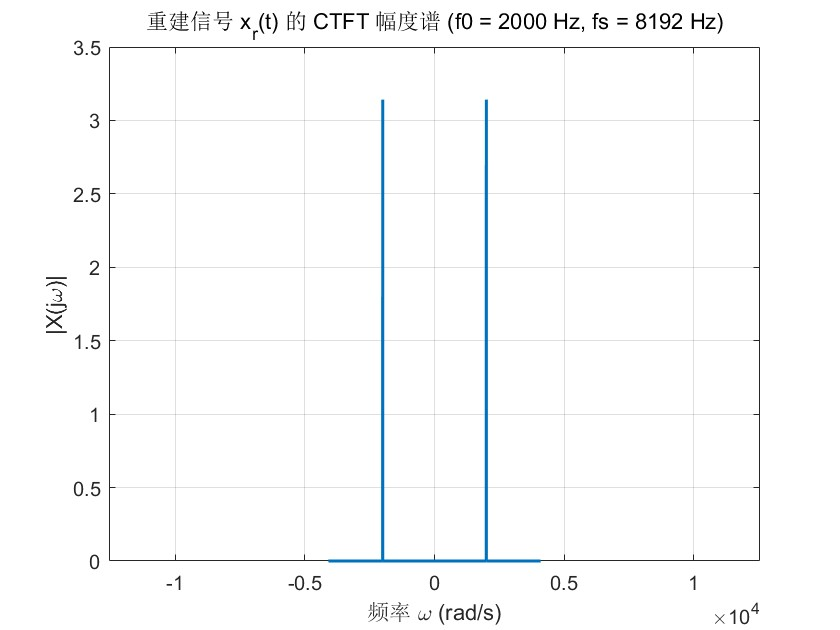
\includegraphics[width=0.6\linewidth]{6.jpg}
\end{figure}

\subsection*{(e) Audio Pitch Test}

When the sampled signals are played using the sound function at $f_s = 8192$ Hz:

\begin{itemize}
    \item The 1500 Hz signal produces a tone at 1500 Hz
    \item The 2000 Hz signal produces a tone at 2000 Hz
    \item The pitch increases as $\Omega_0$ increases
\end{itemize}

This is expected because both frequencies are below the Nyquist frequency, so the reconstructed signal retains the original frequency.

\subsection*{(f) High Frequencies and Aliasing}

Now consider $f_0 = 3500, 4000, 4500, 5000, 5500$ Hz.

The Nyquist frequency is $f_s/2 = 4096$ Hz. When $f_0 > 4096$ Hz, aliasing occurs and the heard frequency is:
$$f_{\text{heard}} = |f_0 - k f_s|, \qquad \text{where } f_{\text{heard}} \leq f_s/2$$

\begin{center}
\begin{tabular}{|c|c|c|c|}
\hline
$f_0$ (Hz) & Aliasing? & $f_{\text{heard}}$ (Hz) & Pitch Change \\
\hline
3500 & No & 3500 & $\uparrow$ \\
4000 & No & 4000 & $\uparrow$ \\
4500 & Yes & $|4500-8192| = 3692$ & $\downarrow$ \\
5000 & Yes & $|5000-8192| = 3192$ & $\downarrow$ \\
5500 & Yes & $|5500-8192| = 2692$ & $\downarrow$ \\
\hline
\end{tabular}
\end{center}

\textbf{Key observation:} As $f_0$ increases from 4500 Hz to 5500 Hz, the heard pitch \emph{decreases} from 3692 Hz to 2692 Hz. This is the classic aliasing effect: high frequencies "fold back" into the low-frequency region.

\begin{figure}[H]
    \centering
    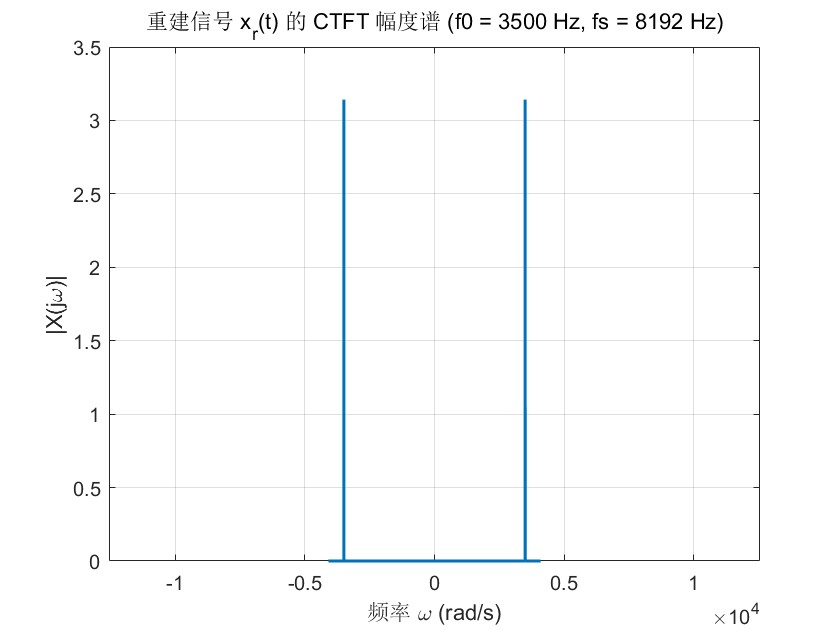
\includegraphics[width=0.6\linewidth]{7.jpg}
\end{figure}

\begin{figure}[H]
    \centering
    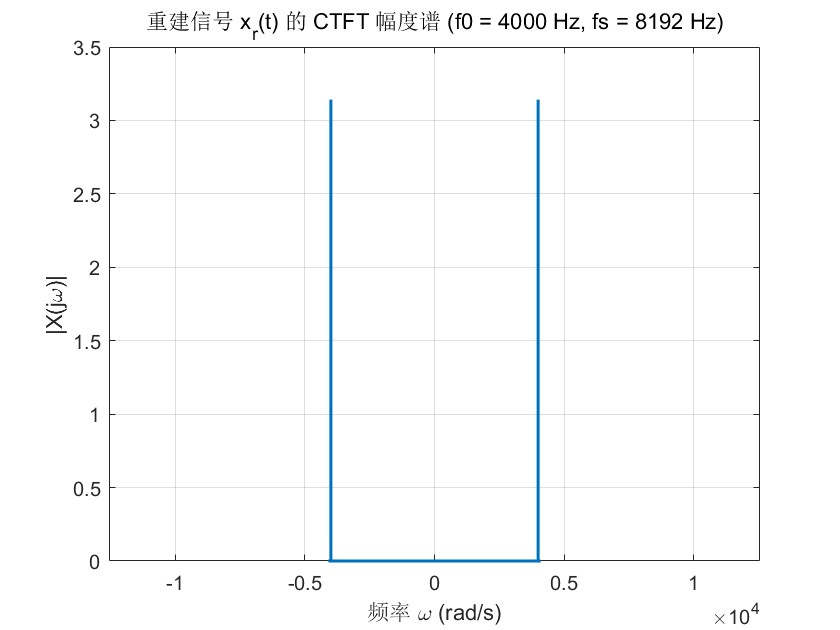
\includegraphics[width=0.6\linewidth]{8.jpg}
\end{figure}

\begin{figure}[H]
    \centering
    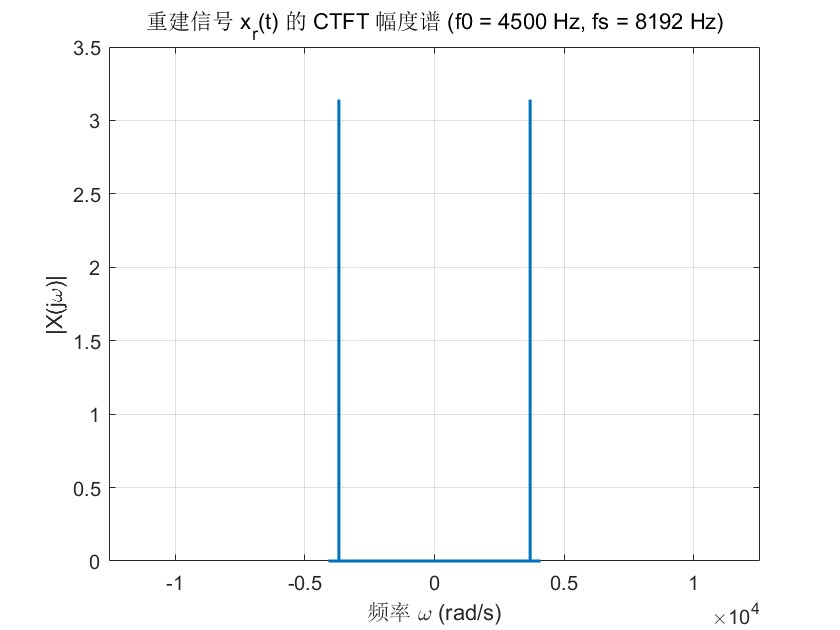
\includegraphics[width=0.6\linewidth]{9.jpg}
\end{figure}

\begin{figure}[H]
    \centering
    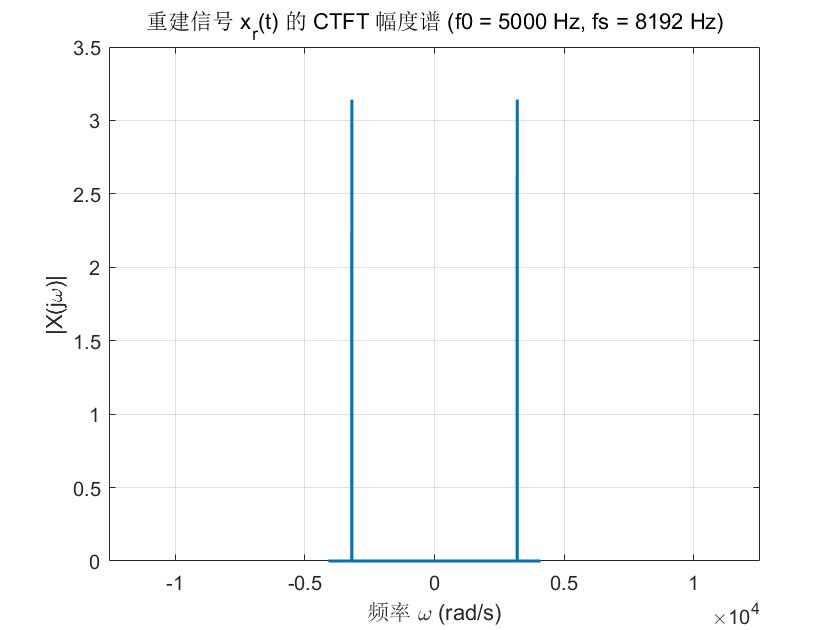
\includegraphics[width=0.6\linewidth]{10.jpg}
\end{figure}
\begin{figure}[H]
    \centering
    
\includegraphics[width=0.6\linewidth]{11.jpg}
\end{figure}


\subsection*{(g) Chirp Signal Sampling}

The chirp signal is defined as:
$$x(t) = \sin\left(\Omega_0 t + \frac{1}{2}\beta t^2\right)$$

with parameters:
$$\Omega_0 = 2\pi(3000) \text{ rad/s}, \qquad \beta = 2000 \text{ rad/s}^2$$

The instantaneous frequency is:
$$\Omega_{\text{inst}}(t) = \frac{d}{dt}\left(\Omega_0 t + \frac{1}{2}\beta t^2\right) = \Omega_0 + \beta t$$

In Hz:
$$f_{\text{inst}}(t) = \frac{\Omega_{\text{inst}}(t)}{2\pi} = 3000 + \frac{2000}{2\pi}t \text{ Hz}$$

For $0 \leq t < 1$ s:
$$3000 \leq f_{\text{inst}}(t) \leq 3000 + \frac{2000}{2\pi} \approx 3318 \text{ Hz}$$

Since the instantaneous frequency remains below $4096$ Hz throughout the interval, \textbf{no aliasing occurs}.

The sampled discrete signal is:
$$x[n] = \sin\left(2\pi \cdot \frac{3000}{8192} \cdot n + \frac{1000}{8192^2} \cdot n^2\right), \qquad n = 0, 1, \dots, 8191$$

\subsection*{(h) Heard Chirp Sound}

When played, the chirp signal produces:
\begin{itemize}
    \item A tone that starts at approximately 3000 Hz
    \item Smoothly rises to approximately 3318 Hz over 1 second
    \item Sounds like a short upward sweep or a bird chirp
\end{itemize}

No abrupt changes occur because the instantaneous frequency remains below the Nyquist frequency throughout the duration.

\subsection*{(i) Predicting Maximum Pitch Time}

For longer durations, the instantaneous frequency will eventually exceed the Nyquist frequency. The maximum audible pitch occurs at the boundary where:
$$f_{\text{inst}}(t) = \frac{f_s}{2} = 4096 \text{ Hz}$$

Solving:
$$3000 + \frac{2000}{2\pi}t = 4096$$
$$t_{\max} = \frac{2\pi(4096 - 3000)}{2000} = \frac{2\pi \cdot 1096}{2000} \approx 3.44 \text{ s}$$

At this time, the instantaneous frequency equals the Nyquist frequency, and the heard pitch reaches its maximum (4096 Hz). Beyond this point, aliasing causes the perceived pitch to decrease.

\subsection*{(j) 10-Second Chirp Analysis}

For $0 \leq t < 10$ s:
$$3000 \leq f_{\text{inst}}(t) \leq 3000 + \frac{2000}{2\pi} \cdot 10 \approx 6183 \text{ Hz}$$

The signal exhibits two distinct phases:

\begin{itemize}
    \item \textbf{Phase 1} ($0 \leq t < 3.44$ s): $f_{\text{inst}} < 4096$ Hz, no aliasing. Pitch rises from 3000 Hz to 4096 Hz.
    \item \textbf{Phase 2} ($3.44 \leq t < 10$ s): $f_{\text{inst}} > 4096$ Hz, aliasing occurs. The heard frequency is:
    $$f_{\text{heard}}(t) = 8192 - f_{\text{inst}}(t) = 8192 - \left(3000 + \frac{2000}{2\pi}t\right)$$
    
    At $t = 10$ s:
    $$f_{\text{heard}}(10) = 8192 - 6183 \approx 2009 \text{ Hz}$$
\end{itemize}

Thus, the overall sound is:
\begin{itemize}
    \item Pitch rises from 3000 Hz to 4096 Hz (first 3.44 s)
    \item Then pitch falls from 4096 Hz to about 2009 Hz (remaining time)
\end{itemize}

The zero-frequency (silence) point is predicted when:
$$f_{\text{inst}}(t) = f_s = 8192 \text{ Hz}$$
$$t_{\text{zero}} = \frac{2\pi(8192 - 3000)}{2000} \approx 16.31 \text{ s}$$



\section*{Problem 2}

This problem explores sinusoidal amplitude modulation (AM) and demodulation of speech signals, including synchronization between transmitter and receiver.

\subsection*{(a) Speech Signal Spectrum}

The speech signal $x(t)$ is loaded from \texttt{origbl.mat}, sampled at $f_s = 8192$ Hz. Its CTFT is computed via FFT:
$$X(f) = \mathcal{F}\{x(t)\}$$

The speech is bandlimited to approximately 1000 Hz:
$$X(f) \approx 0, \quad |f| > 1000 \text{ Hz}$$

\begin{figure}[H]
    \centering
    
\includegraphics[width=0.8\linewidth]{21.jpg}
\end{figure}

\subsection*{(b) AM Modulation}

The modulated signal is:
$$y(t) = x(t) \cos(\omega_c t), \quad \omega_c = 2\pi f_c, \quad f_c = 1500 \text{ Hz}$$

Its spectrum is:
$$Y(f) = \frac{1}{2}\left[X(f - f_c) + X(f + f_c)\right]$$

The spectrum is shifted to $\pm 1500$ Hz.
\begin{figure}[H]
    \centering
    
\includegraphics[width=0.8\linewidth]{22.jpg}
    \end{figure}

\subsection*{(c) Synchronous Demodulation}

With perfect synchronization:
$$w(t) = y(t) \cos(\omega_c t) = x(t) \cos^2(\omega_c t) = \frac{1}{2}x(t) + \frac{1}{2}x(t)\cos(2\omega_c t)$$

Its spectrum:
$$W(f) = \frac{1}{2}X(f) + \frac{1}{4}\left[X(f - 2f_c) + X(f + 2f_c)\right]$$

Lowpass filtering removes the high-frequency components at $\pm 2f_c$, recovering $\frac{1}{2}x(t)$.


\begin{figure}[H]
    \centering
    
\includegraphics[width=0.8\linewidth]{23.jpg}
\end{figure}


\subsection*{(d) Lowpass Filter Design}

The ideal lowpass filter has cutoff frequency $f_c = 1500$ Hz:
$$H(f) = \begin{cases} 1, & |f| \leq f_c \\ 0, & |f| > f_c \end{cases}$$

Impulse response:
$$h(t) = 2f_c \cdot \text{sinc}(2f_c t) = \frac{\sin(2\pi f_c t)}{\pi t}$$

For discrete-time implementation with $L = 41$ taps and sampling period $T_s = 1/f_s$:
$$h[n] = h(nT_s - T), \quad n = 0, 1, \dots, 40$$

where $T = 20/f_s$ is the time shift to make the filter causal.

A Hamming window $w[n]$ is applied:
$$h_w[n] = h[n] \cdot w[n], \quad w[n] = 0.54 - 0.46\cos\left(\frac{2\pi n}{L-1}\right)$$

\begin{figure}[H]
    \centering
    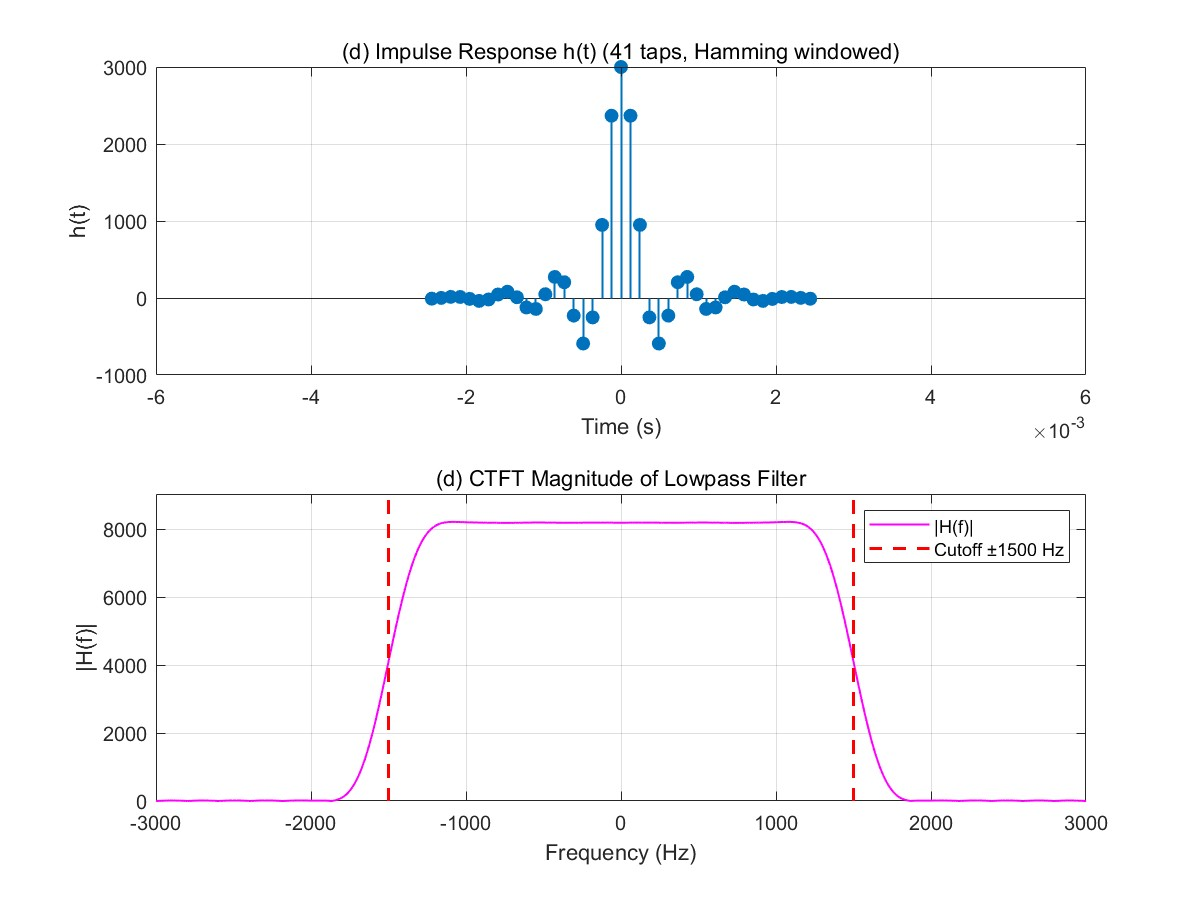
\includegraphics[width=0.8\linewidth]{24.jpg}
\end{figure}

\subsection*{(e) Speech Recovery}

The demodulated signal is filtered:
$$z(t) = w(t) * h(t)$$

After filtering:
$$z(t) \approx \frac{1}{2}x(t)$$

The speech is recovered and played using \texttt{sound(z, fs)}.

\begin{figure}[H]
    \centering
    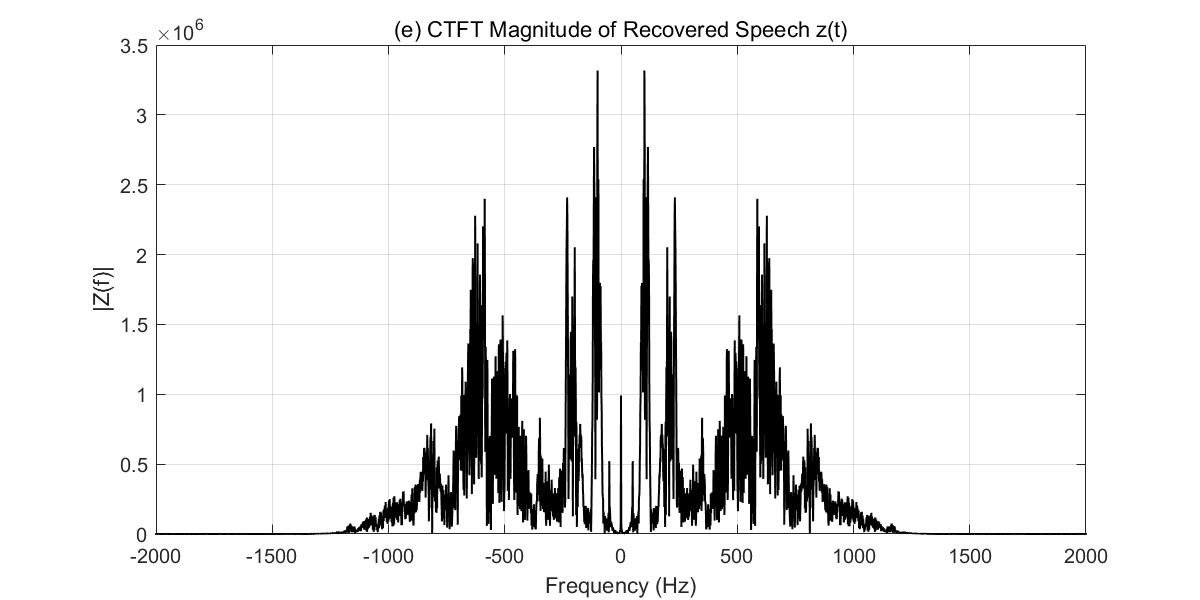
\includegraphics[width=0.8\linewidth]{25.jpg}
\end{figure}
\subsection*{(f) Phase Mismatch Effects}

With phase error $\phi$:
$$w_\phi(t) = y(t) \cos(\omega_c t + \phi) = x(t)\cos(\omega_c t)\cos(\omega_c t + \phi)$$

Using trigonometric identity:
$$w_\phi(t) = \frac{x(t)}{2}\left[\cos(\phi) + \cos(2\omega_c t + \phi)\right]$$

After lowpass filtering:
$$z_\phi(t) = \frac{x(t)}{2}\cos(\phi)$$

\begin{center}
\begin{tabular}{|c|c|c|}
\hline
$\phi$ & $\cos(\phi)$ & Recovered Signal \\
\hline
$0$ & $1$ & $\frac{1}{2}x(t)$ (perfect) \\
$\pi/4$ & $1/\sqrt{2} \approx 0.707$ & $\frac{1}{2\sqrt{2}}x(t)$ (attenuated) \\
$\pi/2$ & $0$ & $0$ (no signal) \\
\hline
\end{tabular}
\end{center}

When $\phi = \pi/2$, the signal is completely lost.


\begin{figure}[H]
    \centering
    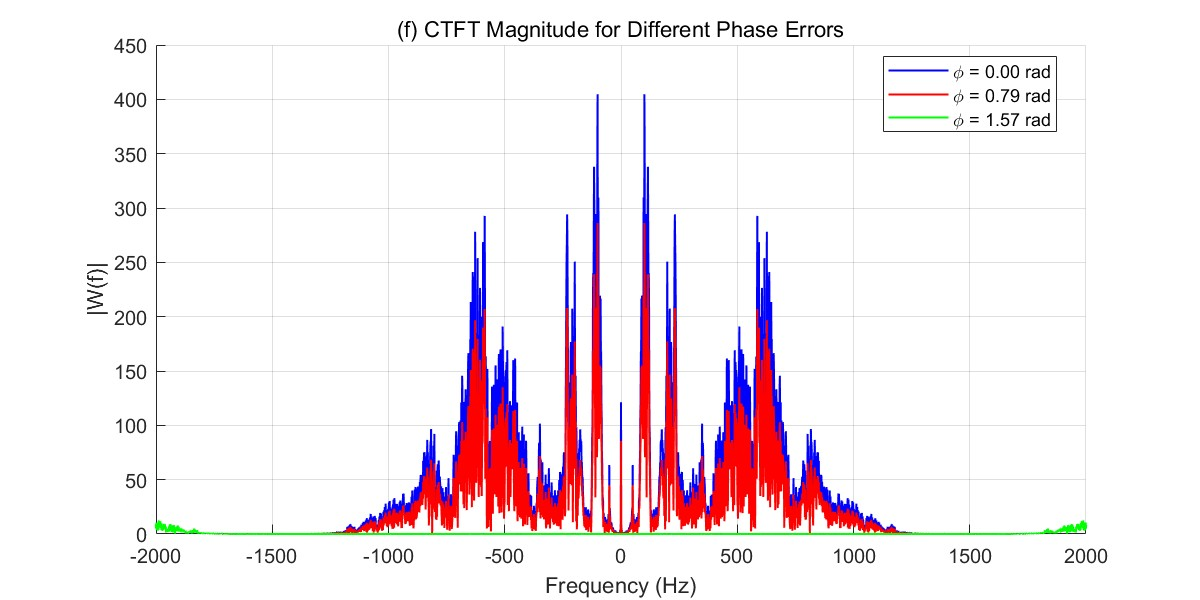
\includegraphics[width=0.8\linewidth]{26.jpg}
\end{figure}


\subsection*{(g) Phase-Locked Loop (PLL)}

A DC offset $A$ is added to ensure $A + x(t) > 0$:
$$y_{\text{PLL}}(t) = (A + x(t)) \cos(\omega_c t + \phi)$$

The PLL estimates the phase $\hat{\phi}(t)$ using:
$$\hat{c}(k) = A \cos(\omega_c t_k + \hat{\phi}_k)$$
$$\hat{\phi}_{k+1} = \hat{\phi}_k + \alpha \big(y_{\text{PLL}}(t_k) - \hat{c}(k)\big)$$

where $\alpha$ is the adaptation step size.

The phase error converges to zero:
$$\lim_{k \to \infty} (\phi - \hat{\phi}_k) \to 0$$

Demodulation using the estimated phase:
$$w_{\text{PLL}}(t) = y_{\text{PLL}}(t) \cos(\omega_c t + \hat{\phi}(t))$$


\begin{figure}[H]
    \centering
    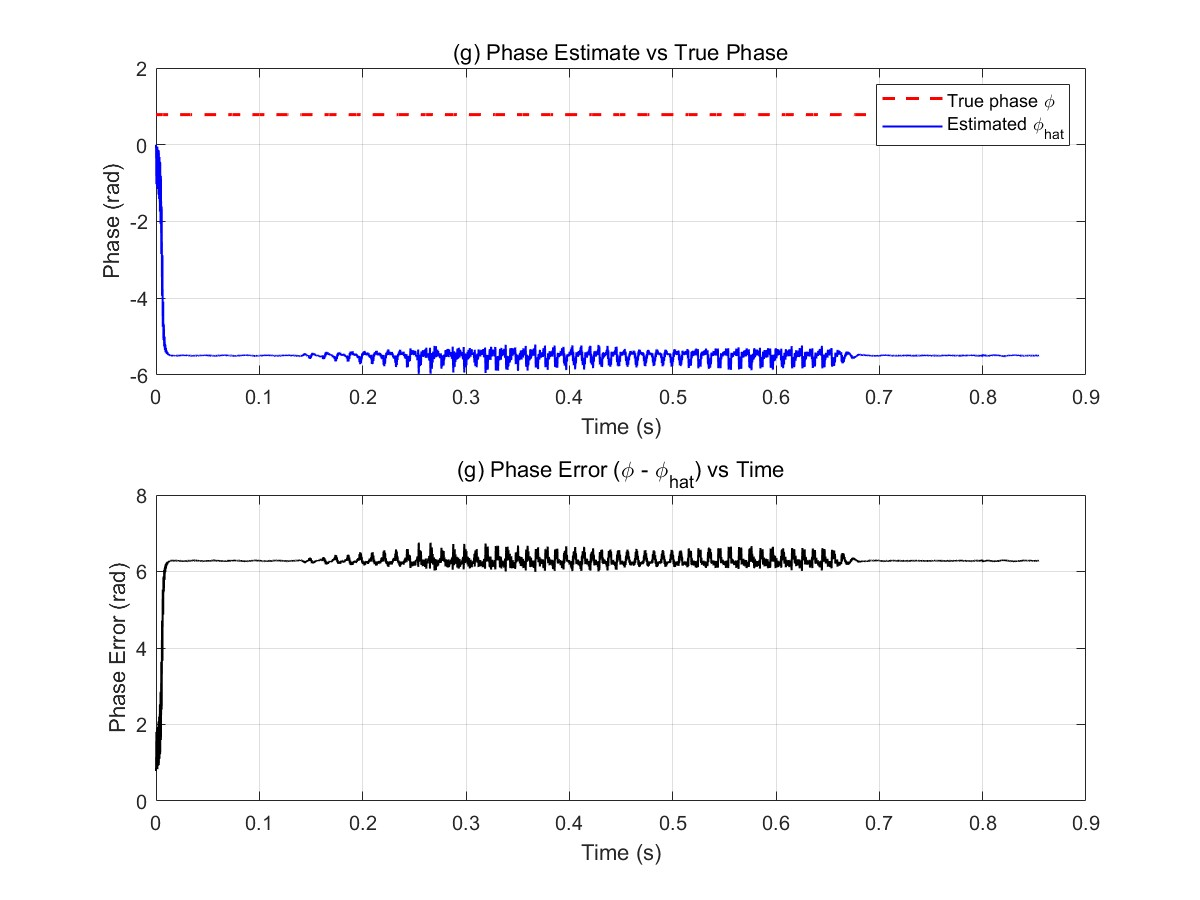
\includegraphics[width=0.8\linewidth]{27.jpg}
\end{figure}
\subsection*{(h) Random Phase Jitter}

The received phase includes random drift:
$$\phi_n = \sum_{i=1}^n \eta_i, \quad \eta_i \sim \mathcal{N}(0, \sigma^2)$$

where $\sigma = 0.01$ is the RMS jitter.

Received signal:
$$y_{\text{jitter}}(t) = (A + x(t)) \cos(\omega_c t + \phi_n)$$

The PLL tracks the phase drift:
$$\hat{\phi}_{n+1} = \hat{\phi}_n + \alpha \big(y_{\text{jitter}}(t_n) - A\cos(\omega_c t_n + \hat{\phi}_n)\big)$$

\subsection*{Parameter Study}

PLL performance depends on:

\begin{enumerate}
    \item \textbf{Adaptation parameter $\alpha$}: Larger $\alpha$ $\Rightarrow$ faster convergence but more noise.
    \item \textbf{Carrier amplitude $A$}: Larger $A$ $\Rightarrow$ stronger signal, easier lock.
    \item \textbf{Phase jitter $\sigma$}: Larger $\sigma$ $\Rightarrow$ harder to track.
\end{enumerate}

\begin{figure}[H]
    \centering
    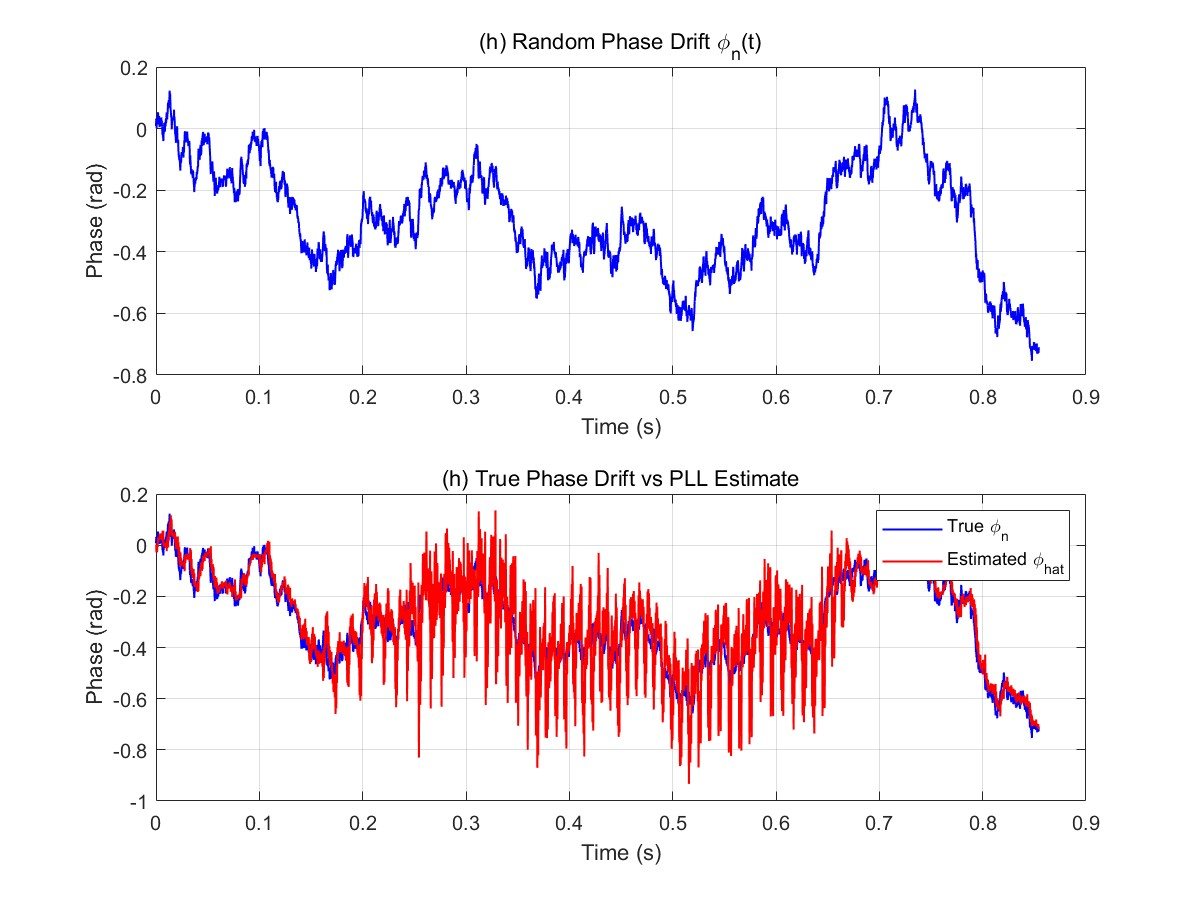
\includegraphics[width=0.8\linewidth]{28.jpg}
\end{figure}

\begin{figure}[H]
    \centering
    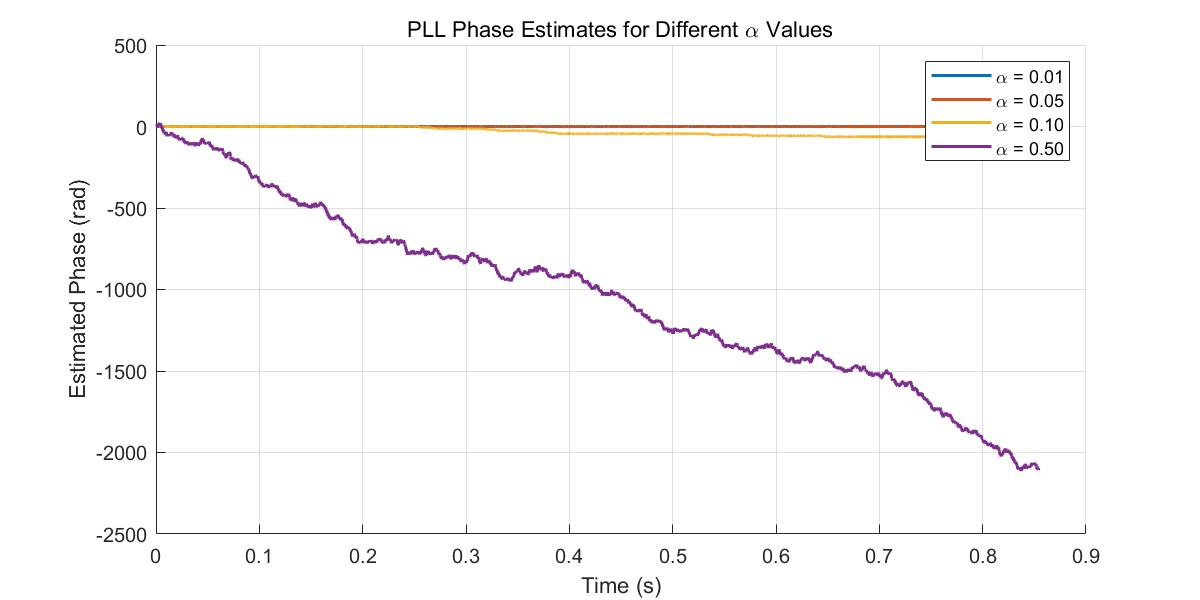
\includegraphics[width=0.8\linewidth]{29.jpg}
\end{figure}

\begin{figure}[H]
    \centering
    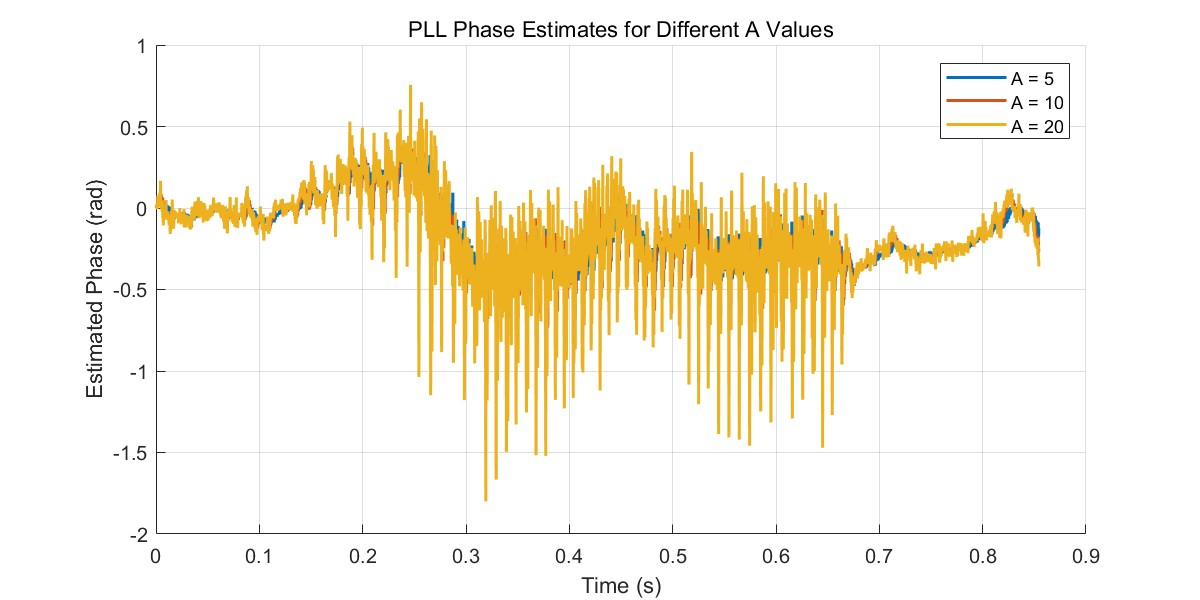
\includegraphics[width=0.8\linewidth]{30.jpg}
\end{figure}

\end{document}